\documentclass[12pt,a4paper]{article}
\usepackage{ctex}
\usepackage{amsmath,amscd,amsbsy,amssymb,latexsym,url,bm,amsthm}
\usepackage{epsfig,graphicx,subfigure}
\usepackage{enumitem,balance}
\usepackage{wrapfig}
\usepackage{mathrsfs,euscript}
\usepackage[usenames]{xcolor}
\usepackage{hyperref}
\usepackage[vlined,ruled,commentsnumbered,linesnumbered]{algorithm2e}
\renewcommand{\algorithmcfname}{算法}
\newtheorem{theorem}{Theorem}
\usepackage{listings}
\newtheorem{lemma}[theorem]{Lemma}
\newtheorem{proposition}[theorem]{Proposition}
\newtheorem{corollary}[theorem]{Corollary}
\newtheorem{exercise}{Exercise}
\newtheorem*{solution}{Solution}
\newtheorem{definition}{Definition}
\theoremstyle{definition}
\definecolor{mygreen}{rgb}{0,0.6,0}
\definecolor{mygray}{rgb}{0.5,0.5,0.5}
\definecolor{mymauve}{rgb}{0.58,0,0.82}
\lstset{
	basicstyle = \footnotesize,       
	breakatwhitespace = false,        
	breaklines = true,                 
	captionpos = b,                    
	commentstyle = \color{mygreen}\bfseries,
	extendedchars = false,   
	keepspaces=true,
	keywordstyle=\color{blue}\bfseries, % keyword style
	language = C++,                     % the language of code
	otherkeywords={string}, 
	numbers=left, 
	numbersep=5pt,
	numberstyle=\tiny\color{mygray},
	rulecolor=\color{black},         
	showspaces=false,  
	showstringspaces=false, 
	showtabs=false,    
	stepnumber=1,         
	stringstyle=\color{mymauve},        % string literal style
	tabsize=2,          
	title=\lstname                      
}
%\numberwithin{equation}{section}
%\numberwithin{figure}{section}

\renewcommand{\thefootnote}{\fnsymbol{footnote}}

\newcommand{\postscript}[2]
{\setlength{\epsfxsize}{#2\hsize}
	\centerline{\epsfbox{#1}}}

\renewcommand{\baselinestretch}{1.0}

\setlength{\oddsidemargin}{-0.365in}
\setlength{\evensidemargin}{-0.365in}
\setlength{\topmargin}{-0.3in}
\setlength{\headheight}{0in}
\setlength{\headsep}{0in}
\setlength{\textheight}{10.1in}
\setlength{\textwidth}{7in}
\makeatletter \renewenvironment{proof}[1][Proof] {\par\pushQED{\qed}\normalfont\topsep6\p@\@plus6\p@\relax\trivlist\item[\hskip\labelsep\bfseries#1\@addpunct{.}]\ignorespaces}{\popQED\endtrivlist\@endpefalse} \makeatother
\makeatletter
\renewenvironment{solution}[1][Solution] {\par\pushQED{\qed}\normalfont\topsep6\p@\@plus6\p@\relax\trivlist\item[\hskip\labelsep\bfseries#1\@addpunct{.}]\ignorespaces}{\popQED\endtrivlist\@endpefalse} \makeatother

\usepackage{listings}

\begin{document}
\noindent

%========================================================================
\noindent\framebox[\linewidth]{\shortstack[c]{
\Large{\textbf{Report}}\vspace{1mm}\\
CS214-Algorithm and Complexity, Spring 2018}}
\begin{center}
\footnotesize{\color{black} Name: 杨培灏  \quad Student ID: 516021910233}
\end{center}

\textbf{问题概述:}介绍决策树模型。
\textbf{算法:}
	决策树内部节点存放对属性的判断,分支为判断输出,叶节点存放类标号也即决策。ID3、C4.5、CART均为决策树的学习算法,它们的差别在于选择的特征不同,具体过程均为一个贪心的求解过程:利用对当前样本集分类能力最小的属性进行分类,缩小样本集,得到规模更小的分类问题。
\begin{enumerate}
	\item{
		\textbf{ID3算法:}
		该算法优先将分类能力最好的属性选作根节点,自顶向下构造决策树。其基本情况为训练样本属于同一类,则直接输出。否则以熵及对应的信息增益为其分裂属性选择的依据。
		
		对于一个随机变量$X$,其熵的计算公式为
		$$H(X)=-\sum{p_i\log p_i}$$
		其中$p_i$为该随机变量取有限不同值的概率(此处用频率作为其概率,即数据集中某个划分的子集的样本数量除以训练集样本总数量)。熵值越大,意味着随机变量的不确定性越强,即在分类时,熵值越大对应的分类时的不确定性越强。条件熵为两个随机变量$X$和$Y$,给定随机变量$X=x_i$后,$Y$在$X=x_i$的条件下的概率分布对应的熵值即为$H(Y|X=x_i)$,那么条件熵为$X$给定条件下$Y$的随机分布对应熵值的数学期望为
		$$H(Y|X)=\sum{p_iH(Y|X_i)}$$
		其中$p_i$为随机变量$X$的不同取值对应的概率,信息增益为得知特征$X$的某信息对于类$Y$的不确定性的减少程度。特征A对训练集D记信息增益为$g(D,A)$
		$$g(D,A)=H(D)-H(D|A)$$
		信息增益大的特征具有更强的分类能力。
		
		\begin{algorithm}
			\caption{ID3()}
			\KwIn{学习样本集合$Example$,样例属性集Character}
			\KwOut{决策树}
			创建树的根节点;\\
			\If{样例均为正}{
				返回标签为正的单节点树;\\
			}\ElseIf{样例均为负}{
				返回标签为负的单节点树;\\
			}
			根据信息增益,求出属性中对样本分类最好的属性$A$;\\
			\For{属性$A$的每一个可能值$v_i$}{
				在根节点下增加分支对应的$A=v_i$的测试结果;\\
				设$Example(i)$为$Example$中满足属性$A$的值为$v_i$的子集;\\
				递归调用ID3(Example(i),Character-\{A\});
			}	
			
		\end{algorithm}
	
		该算法的缺点是使用了信息增益作为判断标准,那么可能会偏向取大量不同值的特征,然而这种特征分类通常是没有意义的。
	} 
	\item{
		\textbf{C4.5算法:}该算法基于信息增益率,信息增益率为信息增益除以当前节点的总熵值,即$g(D,A)/H(D)$。该算法选择了信息增益率作为分裂属性,克服了ID3算法中的通过信息增益而选择拥有更多属性值的属性作为分裂属性的不足。能够处理离散型和连续型的属性类型,方法是对连续型属性进行离散化处理。构造决策树后能进行剪枝操作,能够处理缺失属性值的训练数据。
		其算法与ID3类似,只不过换成了信息增益率。
		该算法的缺点是算法的计算效率较低,同时和之前的ID3算法一样只考虑了条件属性和决策之间的关系,但是并没有考虑条件属性间的关系。
		算法中的其他细节还有连续变量的离散化和剪枝:
		连续型属性属性的离散化处理。当属性A为连续型变量时,为了方便划分,我们可以将当前节点的样本根据属性A的属性值,按升序排序为$(x^{A}_{1},\ldots,x^{A}_{1})$,然后对这个序列进行二分分划,共有(N-1)种二分方法,二分阈值分别为
		$$\theta_i=(x^{A}_{i}+x^{A}_{i+1})/2$$
		如此划分数据集为两个子数据集,计算信息增益、信息增益率。
		剪枝。在构造决策树时,由于我们的构造过程基于训练集,所以会发生过拟合的现象,对训练样本完美拟合但是对测试样本则不理想。C4.5算法可以通过剪枝减少模型的复杂度。剪枝分为预剪枝和后剪枝,预剪枝是在构建决策树的过程中提前终止,这种方法不常用,因为很难确定何时终止;后剪枝是在构建完成后,对置信度不高的节点子树用叶节点代替,叶子节点的类标号用原子树中最频繁的类标号。C4.5使用PEP剪枝法,由剪枝前后的错误率来判定是否进行子树的修剪,不需要单独的剪枝数据集。对于一个叶子节点,它覆盖了n个样本,其中有e个错误,那么该叶子节点的错误率为$(e+0.5)/n$,其中0.5为惩罚因子。对于一棵子树,它有L个叶子节点,那么该子树的误判率为
		$$ErrorRatio=\frac{\sum_{i=1}^{L}e_i+0.5L}{\sum_{i=1}^{L}n_i}$$
		假设一棵子树错误分类一个样本取值为1,正确分类一个样本取值为0,则子树的误判次数可以视作一个伯努利分布,可以得到该子树的误判次数的均值和标准差为
		$$ErrorMean=ErrorRatio\times\sum_{i=1}^{L}n_i$$
		$$ErrorSTD=\sqrt{ErrorRatio\times\sum_{i=1}^{L}n_i\times(1-ErrorRatio)}$$
		将子树替换成叶子节点后,该叶子节点的误判率为:
		$$ErrorRatio'=\frac{\sum_{i=1}^{L}e_i+0.5}{\sum_{i=1}^{L}n_i}$$
		$$ErrorMean'=ErrorRatio'\times\sum_{i=1}^{L}n_i$$
		剪枝的条件为
		$$ErrorMean+ErrorSTD\ge ErrorMean'$$
	}
	\item{
		\textbf{CART算法:}该算法基于基尼指数,可以运用在连续的变量的情况。。CART构造出的决策树一定是二叉树,内部节点的特征的取值为“是”和“否”,左分支取值“是”,右分支取值“否”。这样的决策树等价于递归地二分每个特征,将输入空间划分为有限个单元,并在这些单元上确定预测的概率分布,也就是在输入给定条件下输出的条件概率分布。该算法主要有两步:
		\begin{enumerate}
			\item{决策树生成:生成的决策树要尽可能地大}
			\item{决策树剪枝:对生成的决策树进行剪枝选择最优子树,损失函数最小作为剪枝的标准}
		\end{enumerate}
		决策树的生成过程与前两种相近,不同点在于遇到多属性值(属性值种类大于2)时,将多属性值的属性分为两组,根据不同分组计算基尼指数增益,选择增益最大的分组作为该属性属性值的分组。在所有属性中,选择基尼指数增益最大的属性进行分类。
		记对当前数据集合$D$的划分为$D_1$和$D_2$,则基尼指数为
		$$Gini=1-(\frac{D_2}{D})^2-(\frac{D_2}{D})^2$$
		在某属性条件$A$下,基尼指数为记作D(A),则其基尼指数增益为
		$$g(D,A)=Gini-Gini(A)$$
		同样增益强的属性具有更好的分类能力,而剪枝方法与前面提到的方法相似。
	}
\end{enumerate}
\textbf{实际问题:}
	利用决策树解决眼镜配制的问题。输入数据如下。
	\begin{center}
		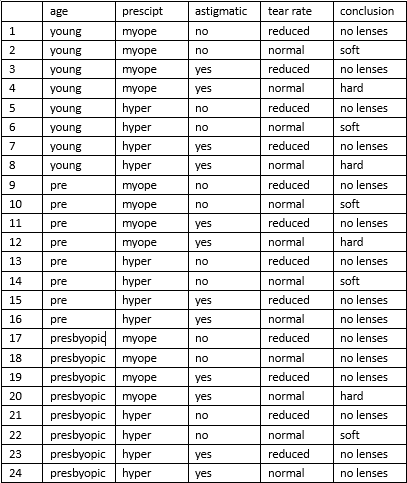
\includegraphics[width=0.75\textwidth]{static.png}
	\end{center}

\textbf{代码实现:}
	见附页,实现了ID3和C4.5两种算法。
	
\textbf{求解输出:}
	图片中训练时建立的决策树的部分,每行第一个数为上一层分裂属性的值,第二个为该节点的分裂属性(叶节点则省略),第三个为当前节点剩余的样本数。
	首先是ID3算法,如果使用全部数据来训练
	\begin{center}
		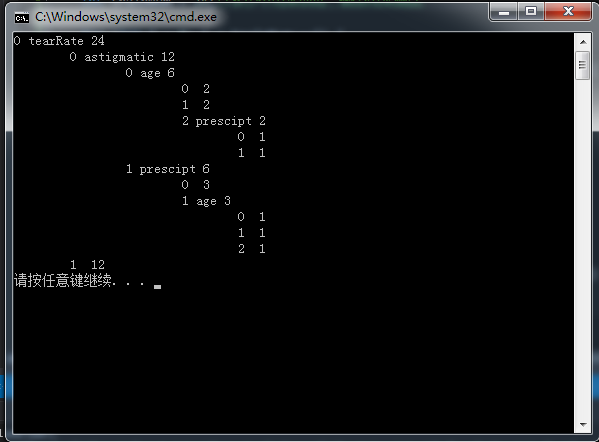
\includegraphics[width=\textwidth]{ID3all2train.png}
	\end{center}
	如果使用前18行数据来训练,后六行测试
	\begin{center}
		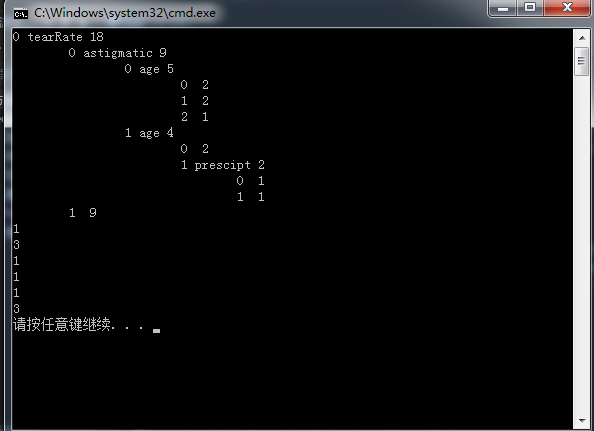
\includegraphics[width=\textwidth]{ID18toTrain.png}
	\end{center}
	接下来是C4.5算法,如果使用全部数据来训练
	\begin{center}
		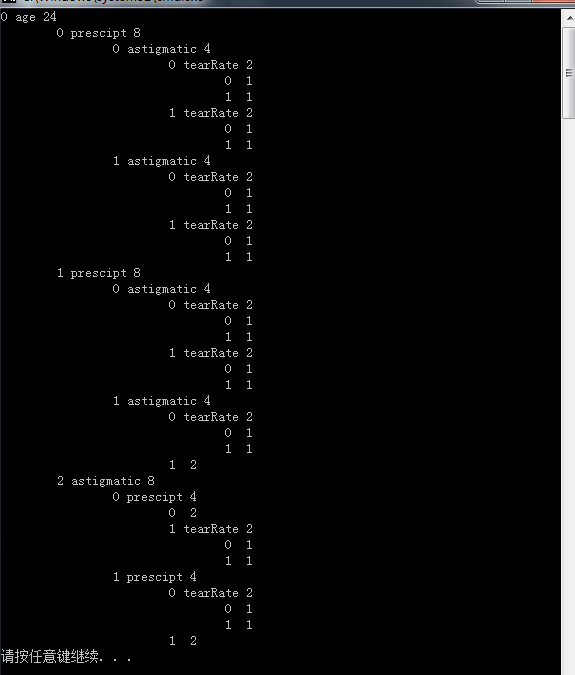
\includegraphics[width=\textwidth]{C45all2train.png}
	\end{center}
	如果使用前18行数据来训练,后六行测试
	\begin{center}
		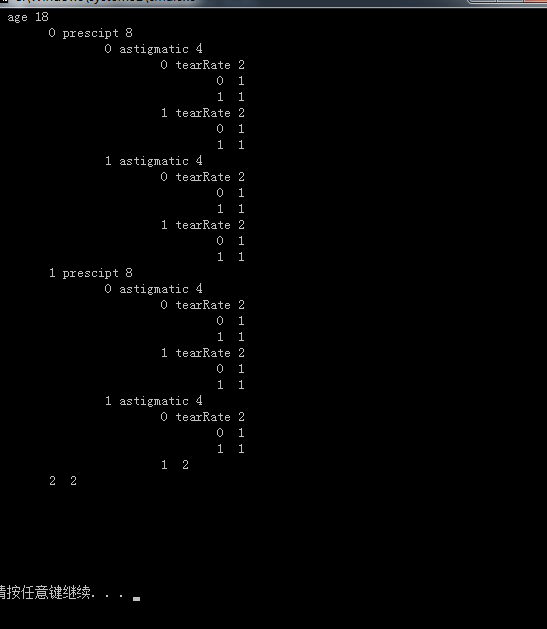
\includegraphics[width=\textwidth]{C18toTrain.png}
	\end{center}
%========================================================================
\end{document}
